

%\begin{comment}
\section{Data Quality and Stability Checks}
%\textbf{\textcolor{red}{Yet to be fleshed out.}}
With an available set of good  event/electron selection cuts, beam charge (measured by Faraday cup) normalized total event counts (sometimes also known as event ``yield''), as well as polarization dependent %polarized count 
differences, were calculated for each of the data files for all the runs %run numbers 
and then plotted against the run number to study the data quality and stability as shown by Figs. \ref{figyldTot}, \ref{figyldDiff} and \ref{figrstADCs}.

If nothing unusual happened or if the experimental conditions are not changed, %between the data taking, 
then it is expected that the event yield as well as the count differences remain constant over time. Therefore, the graphs of these event counts plotted versus time or run number (which also roughly reflect the flow of time) should indicate the stability and quality of the data collected. For example, Fig. \ref{figyldTot} shows such a total yield plot for all the data files from the 2.0 GeV beam energy data set on deuteron target. We can see that these data runs display %quite 
 some features of instability over the full period of time, but %some degree of SEK
 stability over short time periods. For example, all the data with run numbers below about 51610 show significantly higher event yield than the runs after that run %. This could have been due to  and it suddenly drops after around that run number 
 (possibly due to  beam-target misalignment %that could have happened due to target replacement activity).
 as indicated by raster magnet ADC values in Fig \ref{figrstADCs}. 



Likewise, the stability of the polarized %total %GED
count differences in the elastic region ($0.9$ GeV $<W<1.0$ GeV) as well as separately in the delta ($\Delta$) resonance region were studied by plotting them versus the same run numbers (here the elastic and $\Delta$-resonance regions are %should be 
considered separately, because the spin asymmetries in these two regions have opposite signs, which would 
%otherwise cancel each other's effects in the total count difference. %, thus not allowing us any instability to be seen if they existed). 
have decreased the observed difference if combined.
To further enhance the sensitivity of the observation, the difference of the count differences measured in the elastic and $\Delta$-resonance regions as given by 

\begin{eqnarray}
\label{eqPolED}
\Delta N_{elastic} - \Delta N_{\Delta-res} = \frac{1}{P_b P_t} \left[ \left( \frac{N^+}{FC^+} - \frac{N^-}{FC^-} \right)_{elastic} -   \left( \frac{N^+}{FC^+} - \frac{N^-}{FC^-} \right)_{\Delta} ~ \right]
\end{eqnarray}
were plotted (see Fig. \ref{figyldDiff}). It was observed %, to our delight, 
that this elastic normalized count difference (which is what really matters to our analysis, in the end) was much more stable than the total yield.

%http://amath.colorado.edu/documentation/LaTeX/reference/figures.html
\begin{figure} [H] %[h] %ht, htpb (p - float, b = bottom, h=? t = top)
%\leavevmode \includegraphics[width=0.6\textwidth]{chap6expSetup/Figures/cebaf.eps}  %0.6 is the fraction of the real image width????
  %\leavevmode \includegraphics[width=0.9\textwidth]{FigQualCheckBkGrnd/totYld_2_2.eps}  %0.6 is the fraction of the real image width????
  \leavevmode \includegraphics[width=0.9\textwidth]{TexmakerMyFinTh/FigQualCheckBkGrnd/totYld_2_2.png}  %0.6 is the fraction of the real image width????
  \caption[Normalized total yield (2.0 GeV (ND$_3$))]{Total normalized yield ($= \frac{N^+ + N^-}{FC^+ + FC^-}$) for 2.0 GeV ND$_3$ runs.}
  \label{figyldTot}
\end{figure}



\begin{figure}[H] %[h] %ht, htpb (p - float, b = bottom, h=? t = top)
  %\leavevmode \includegraphics[width=0.9\textwidth]{FigQualCheckBkGrnd/yldDiffnormED_2_2.eps} 
  \leavevmode \includegraphics[width=0.9\textwidth]{TexmakerMyFinTh/FigQualCheckBkGrnd/yldDiffnormED_2_2.png} 
  \caption[$\Delta N$ for elastic minus $\Delta$-resonance]{Polarized yield differences (Eq. \ref{eqPolED}) normalized with $P_bP_t$ and BPM/F-cup for elastic peak minus that for the $\Delta$ peak for the 2.0 GeV \nd3 runs.}
  \label{figyldDiff}
\end{figure}

The same was also repeated for the other variables such as the root-mean-square of the ADC values (see Fig. \ref{figrstADCs}) which carry information on the X and Y coordinates of the beam at the interaction vertex, thus their plots giving us somewhat more direct information on whether there was any misalignment between the beam and the target.

\begin{figure}%[h] %ht, htpb (p - float, b = bottom, h=? t = top)
  %\leavevmode \includegraphics[width=1.0\textwidth]{FigQualCheckBkGrnd/rmsRastAdcVRun2_2.eps} 
  \leavevmode \includegraphics[width=1.0\textwidth]{TexmakerMyFinTh/FigQualCheckBkGrnd/rmsRastAdcVRun2_2.png} 
  \caption[RMS of raster ADCs]{Root-mean-square of the ADC values for the raster magnet currents in the directions %arms 
  X and Y. The distributions show a larger raster size in the y-direction for the first group of runs, indicating that the beam may have been hitting the edges and the walls of the target or other more dense structure support materials, thus explaining the higher total yield for the corresponding runs as shown by the Fig. \ref{figyldTot}. This does not affect our final analysis because these off-target materials are not polarized and, hence, do not contribute to the polarization dependent count difference ($\Delta N$) used in the final analysis.}
  \label{figrstADCs}
\end{figure}

Based on the  studies of these quality and stability plots, the data runs were divided into subgroups with each beam energy data set. In each subgroup, the data showed more stability than over the whole run period for the given beam energy. For example, in case of the 2.0 GeV deuteron data, the runs were divided into four distinct sub groups corresponding to the four separate bands as seen in the Fig. \ref{figyldTot}. These subgroups were later treated and analyzed separately to get the corresponding normalized polarized count differences (with all data runs from each subgroup combined together). After the initial combination within the subgroups, they were again combined into the grand total by properly considering the half-wave-plate status, and the target polarization directions.

%\end{comment}



\begin{comment} %Already commented (on my thesis version)
%\usepackage{verbatim} % For multiline comments: http://www.devdaily.com/blog/post/latex/multi-line-comments-in-latex-begin-123-comment-125-verbatim
\kpb
  Figures (fig~(\ref{figTRvI_ls})) and (fig~(\ref{figYldvTR_l}))
% http://texblog.wordpress.com/2007/08/01/placing-figurestables-side-by-side-minipage/
\begin{figure}[ht]
\begin{minipage}[b]{0.5\linewidth}
\centering
\includegraphics[scale=0.4]{FigQualCheckBkGrnd/trRateVIb_lumScanRuns.eps}
%\caption{default}
 \caption[Trigger rate]{Trigger rate versus beam current for 1.3 GeV luminosity-scan runs (6 runs) showing that the rate is proportional to the current or luminosity general.}
\label{figTRvI_ls}
\end{minipage}
\hspace{0.5cm}
\begin{minipage}[b]{0.5\linewidth}
\centering
\includegraphics[scale=0.4]{FigQualCheckBkGrnd/yldVtrRateTh0_lumScanRuns.eps}
  \caption[Yield of 1.3 GeV luminosity scans]{Normalized yield vs the trigger rate for the 1.3 GeV luminosity-scan runs (6 runs) showing that the detection efficiency decreases with the rate at which the events occur (i.e., the trigger rate or effectively the luminosity).}
%\caption{default}
\label{figYldvTR_ls}
\end{minipage}
\end{figure}
\kpe




\begin{figure}
\centering
%The following \mbox{} gives the overfull \hbox warning
\mbox{\subfigure{\includegraphics[width=3in]{FigQualCheckBkGrnd/trRateVIb_lumScanRuns.eps}}\quad
\subfigure{\includegraphics[width=3in]{FigQualCheckBkGrnd/yldVtrRateTh0_lumScanRuns.eps} }}
\caption[Trigger Rate]{( \textbf{Left}: Trigger rate versus beam current for 1.3 GeV luminosity-scan runs (6 runs) showing that the rate is proportional to the current or luminosity. \textbf{Right}: Normalized yield vs the trigger rate for the 1.3 GeV luminosity-scan runs (6 runs) showing that the detection efficiency decreases with the rate at which the events occur (i.e., the trigger rate or effectively the luminosity).} 
\label{figlsPlts}
\end{figure}

%Note that for JPEG images the graphics package is required: \usepackage{graphics}

\begin{figure}[htpb] %ht, htpb (p - float, b = bottom, h=? t = top)
  \leavevmode \includegraphics[width=1.0\textwidth]{FigQualCheckBkGrnd/yldVtrRateTh0_2_2.eps} 
  \caption[Yield vs Trigger Rate]{Normalized yield vs the trigger rate within 6-10$^o$ of $\theta$ for the first of the three sets of 2.3 GeV \nd3 runs showing the drop of detection efficiency with the trigger rate.}
  \label{figYldvTR_22}
\end{figure}



\begin{figure}[htpb] %ht, htpb (p - float, b = bottom, h=? t = top)
  %\leavevmode \includegraphics[width=1.0\textwidth]{FigQualCheckBkGrnd/Eff_vs_Lumi_EG4.eps} %For some reason this email-downloaded-copy didn't work 
  %Looks like that is a acrobat-reader problem
  \leavevmode \includegraphics[width=1.0\textwidth]{FigQualCheckBkGrnd/Eff_vs_Lumi_EG4convert.eps} 
  \caption[Fit parameter ratios vs Bin Numbers]{Ratio of fit parameters (slope/offset) plotted against the three bin numbers, where the parameters are from the various linear fits to the normalized yields vs trigger rates such as . The average of the 7 ``good'' curves (black) can be used to correct data and the ``error bars'' (the 1-sigma deviation) as a systematic error.(Plot courtesy of S. Kuhn).}
  \label{figpRatioVthBin}
\end{figure}

\end{comment}  %Already commented (on my thesis version)

%\end{comment} 
